\FloatBarrier
\section{Дополнительные проверки}

После просмотра исходного test добавлены повторения полного банка,
проверка бюджета и эксперименты на другом периоде и новых пользователях.
Перед новыми запусками сохранён \code{artifacts/additional/plan.lock.json}.
Они дополняют исходное сравнение, его признаки и метрики не менялись

\subsection{Почему отбор уступил полному банку}

На тех же train, search и confirm сопоставлены три фиксированных
набора признаков при лимитах 180 и 450 деревьев, каждый с тремя seed.
На search полный банк превосходил отобранный набор уже при 180 деревьях
на 0.00706 \([+0.00418,+0.01004]\)

\begin{table}[!htbp]
\centering
\small
\setlength{\tabcolsep}{4pt}
\setlength{\reporttablewidth}{\dimexpr\linewidth-32pt\relax}
\begin{tabular}{@{}>{\raggedright\arraybackslash}p{0.17000\reporttablewidth}>{\raggedright\arraybackslash}p{0.12000\reporttablewidth}>{\raggedright\arraybackslash}p{0.25000\reporttablewidth}>{\raggedright\arraybackslash}p{0.23000\reporttablewidth}>{\raggedright\arraybackslash}p{0.23000\reporttablewidth}@{}}
\toprule
Часть & Лимит & Ручной набор & Автоотбор & Полный банк \\
\midrule
search & 180 & 0.49706 & 0.50836 & 0.51542 \\
search & 450 & 0.50497 & 0.51525 & 0.52351 \\
confirm & 180 & 0.48322 & 0.50008 & 0.51026 \\
confirm & 450 & 0.49035 & 0.50371 & 0.51621 \\
\bottomrule
\end{tabular}
\caption{NDCG@10 ансамблей трёх seed при лимитах 180 и 450 деревьев}
\label{tab:kion-budget}
\end{table}

На confirm изменение разности «банк минус отбор» при переходе
от 180 к 450 деревьям составило 0.00232
\([-0.00064,+0.00522]\). Интервал включает ноль,
поэтому объяснить проигрыш только коротким бюджетом нельзя

Ограничение самого поиска состоит в том, что он проверяет отдельные группы
и объединения лучших двух и трёх, но не рассматривает весь банк
как отдельного кандидата. Полезность группы в сочетании с другими
может быть пропущена. Важность признака в CatBoost описывает его
использование моделью и сама по себе не доказывает пользу включения в набор

\subsection{Другой период и новые пользователи}

Для более ранней тестовой недели, с 26 июля по 1 августа, сохранены те же
30\,000 пользователей. Отбор повторён на более раннем search,
параметры \code{depth=6} и \code{l2_leaf_reg=3} перенесены без нового подбора.
Выбраны \code{window_1d}, \code{window_3d} и \code{multigenre},
всего 71 признак

Отдельно с seed 2027 равномерно выбраны 5\,000 пользователей,
не входивших в основную когорту. Сохранены все 28\,907 их записей.
Модели обучены и признаки отобраны заново только на историях новой когорты.
Выбраны \code{multigenre}, \code{decay_30d} и \code{decay_2d},
всего 63 признака. В её test 1\,308 запросов у 838 пользователей

\begin{table}[!htbp]
\centering
\small
\setlength{\tabcolsep}{4pt}
\setlength{\reporttablewidth}{\dimexpr\linewidth-24pt\relax}
\begin{tabular}{@{}>{\raggedright\arraybackslash}p{0.43000\reporttablewidth}>{\raggedright\arraybackslash}p{0.19000\reporttablewidth}>{\raggedright\arraybackslash}p{0.19000\reporttablewidth}>{\raggedright\arraybackslash}p{0.19000\reporttablewidth}@{}}
\toprule
Тестовая выборка & Ручной набор & Автоотбор & Полный банк \\
\midrule
16-22 августа, 30\,000 & 0.47332 & 0.48440 & 0.49544 \\
26 июля - 1 августа, 30\,000 & 0.49704 & 0.51714 & 0.51603 \\
16-22 августа, новые 5\,000 & 0.43819 & 0.45044 & 0.45642 \\
\bottomrule
\end{tabular}
\caption{NDCG@10 на смешанных кандидатах, в каждом опыте ансамбли трёх seed}
\label{tab:kion-replication}
\end{table}

На более ранней неделе прирост автоотбора к ручному набору равен 0.02011
\([+0.01648,+0.02388]\). Разность полного банка и автоотбора составляет
\(-0.00111\) \([-0.00366,+0.00115]\).
На новых пользователях прирост автоотбора к ручному набору равен
0.01226 \([+0.00372,+0.02082]\)

При равномерных контролях в новой когорте ручной набор получает
0.61485, автоотбор 0.61398. Разность \(-0.00087\)
\([-0.00912,+0.00767]\) не подтверждает преимущество отбора.
В обеих дополнительных выборках интервалы разности полного банка
и популярности на полном каталоге также включают ноль

Временная проверка ретроспективна: используются те же пользователи,
часть ранних событий входила в обучение исходного опыта.
Новая когорта отделена по пользователям, но сохраняет общий источник,
объекты и календарный период. Дополнительные сравнения носят
исследовательский характер, поправка на множественные проверки не применялась

\begin{figure}[!htbp]
\centering
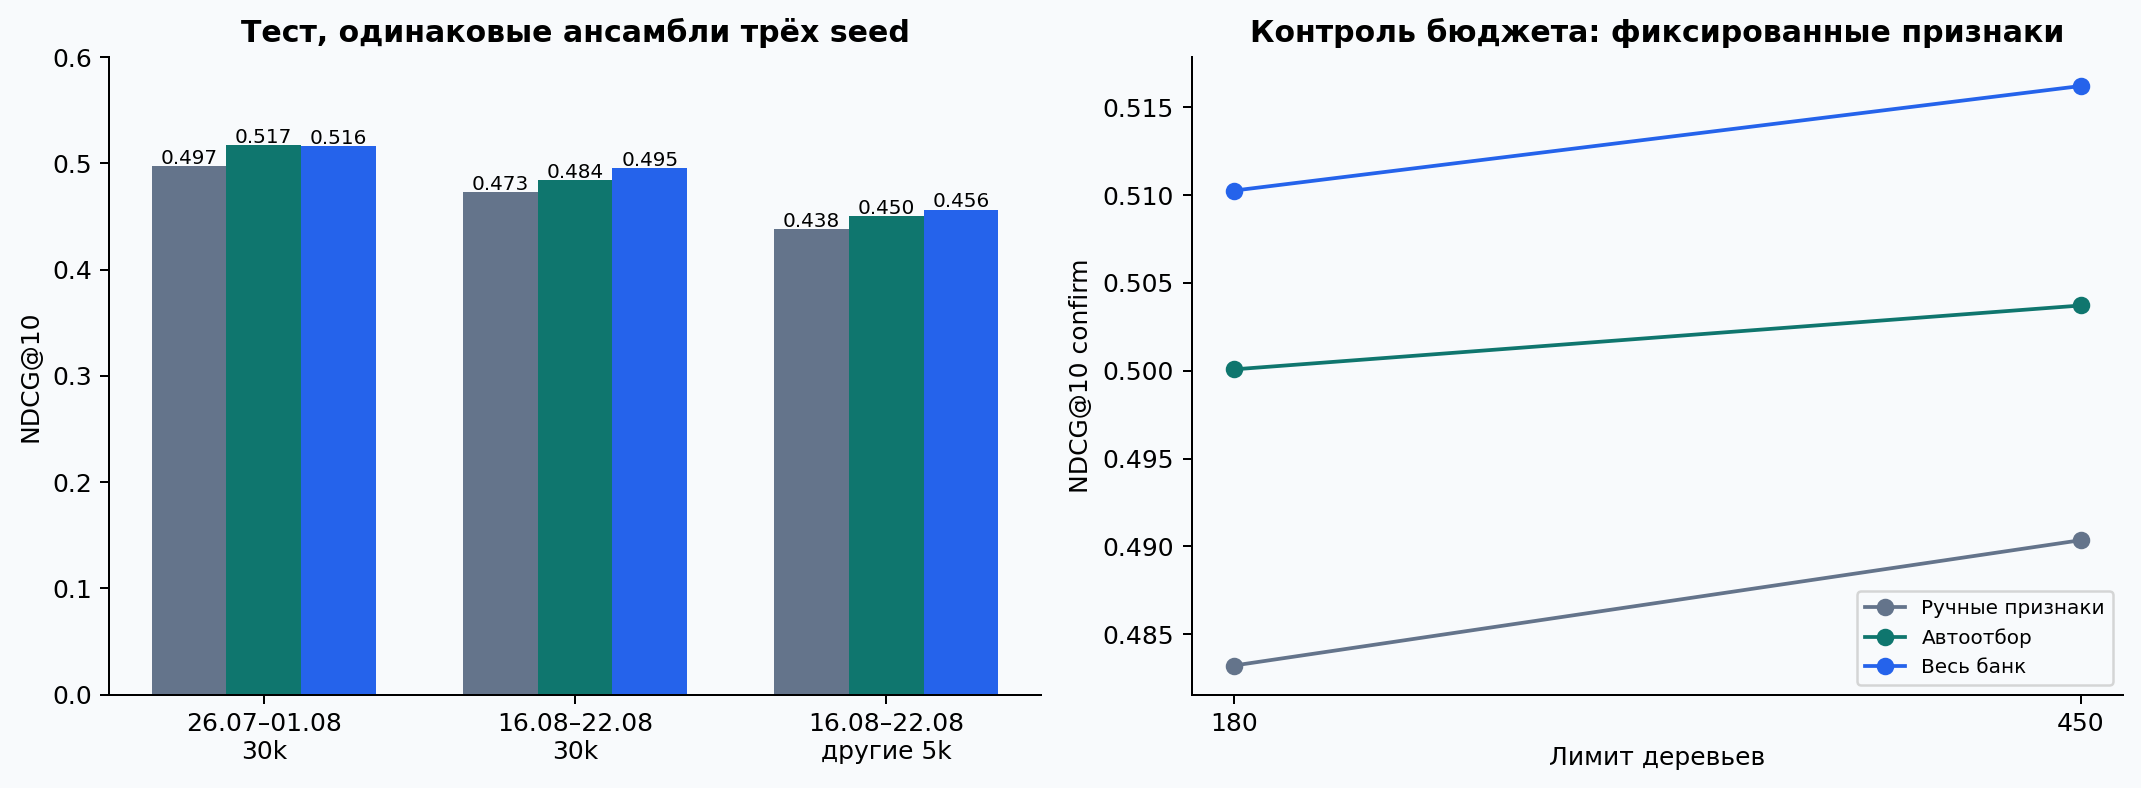
\includegraphics[width=\linewidth,height=.31\textheight,keepaspectratio]{figures/followup.png}
\caption{Сравнение трёх наборов по периодам и когортам, справа влияние лимита деревьев на confirm}
\label{fig:kion-followup}
\end{figure}
